{\color{indiagreen}\subsection{Moč}}
\begin{align*}
	P &= \frac{A}{t}[1\frac{J}{s} = 1W] \rightarrow \text{wat}\\
	1kwh = 10^3 \frac{J}{\cancelto{}{s}} * 3600\cancelto{}{s}&= 3,6*10^6 J \rightarrow \text{enota za {\color{bostonuniversityred}delo}}\\ 
\end{align*}
Če na telo deluje sila:\\
\begin{align*}
	P &= \frac{\Delta A}{\Delta t}\\
	\Delta A &= F\Delta s\\
	\Delta s &= v\Delta t \rightarrow \text{če je dovolj majhen interval(vrednost)}\\
	P &= \frac{Fv\cancelto{}{\Delta t}}{\cancelto{}{\Delta t}}\\
	P &= Fv\\
\end{align*}
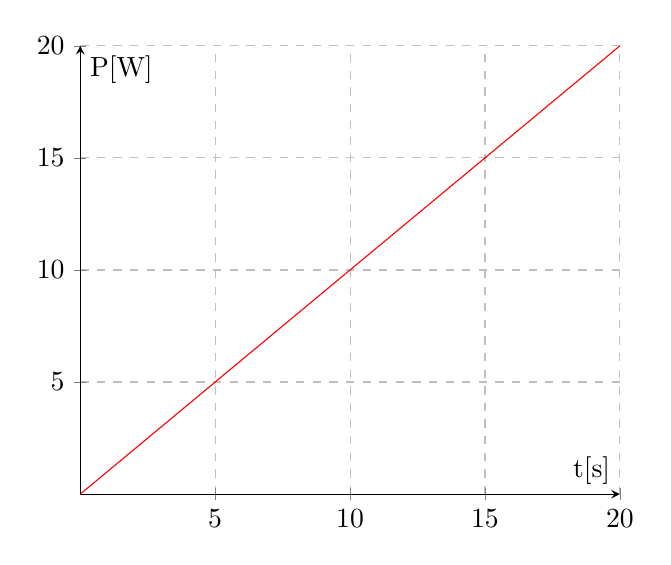
\begin{tikzpicture}
	\begin{axis}[
	    xlabel={t[s]},
	    ylabel={P[W]},
	    xmin=0, xmax=20,
	    ymin=0, ymax=20,
	    xtick={0,5,10,15,20},
	    ytick={0,5,10,15,20},
	    ymajorgrids=true,
	    xmajorgrids=true,
	    grid style=dashed,
	    axis lines=middle,
	]
	 
	\addplot[domain=0:20,red] {x};

	\end{axis}
\end{tikzpicture}
